\documentclass[paper=a4,UTF8,fontsize=11pt]{scrartcl} % A4 paper and 11pt font size
\usepackage[noend]{algpseudocode}
\usepackage{ctex}
\usepackage[T1]{fontenc} % Use 8-bit encoding that has 256 glyphs
\usepackage{fourier} % Use the Adobe Utopia font for the document - comment this line to return to the LaTeX default
\usepackage[english]{babel} % English language/hyphenation
\usepackage{amsmath,amsfonts,amsthm} % Math packages
\usepackage[english]{babel}
\usepackage[utf8]{inputenc}
\usepackage{indentfirst}
\usepackage{algorithm}
\usepackage{lipsum} % Used for inserting dummy 'Lorem ipsum' text into the template
\usepackage{float}
\usepackage{sectsty} % Allows customizing section commands
\allsectionsfont{\centering \normalfont\scshape} % Make all sections centered, the default font and smaıll caps
\usepackage{graphicx}
\usepackage{fancyhdr} % Custom headers and footers
\pagestyle{fancyplain} % Makes all pages in the document conform to the custom headers and footers
\fancyhead{} % No page header - if you want one, create it in the same way as the footers below
\fancyfoot[L]{} % Empty left footer
\fancyfoot[C]{\thepage} % Empty center footer
\fancyfoot[R]{} % Page numbering for right footer
\renewcommand{\headrulewidth}{0pt} % Remove header underlines
\renewcommand{\footrulewidth}{0pt} % Remove footer underlines
\setlength{\headheight}{13.6pt} % Customize the height of the header
\usepackage[noend]{algpseudocode}
\numberwithin{equation}{section} % Number equations within sections (i.e. 1.1, 1.2, 2.1, 2.2 instead of 1, 2, 3, 4)
\numberwithin{figure}{section} % Number figures within sections (i.e. 1.1, 1.2, 2.1, 2.2 instead of 1, 2, 3, 4)
\numberwithin{table}{section} % Number tables within sections (i.e. 1.1, 1.2, 2.1, 2.2 instead of 1, 2, 3, 4)
\usepackage{color}
\setlength\parindent{0.3pt} % Removes all indentation from paragraphs - comment this line for an assignment with lots of text
\usepackage{graphicx}
\usepackage{xcolor}
\usepackage{listings}
\definecolor{mygreen}{rgb}{0,0.6,0}
\definecolor{mygray}{rgb}{0.5,0.5,0.5}
\definecolor{mymauve}{rgb}{0.58,0,0.82}

\lstset{ 
  language=C++,
  backgroundcolor=\color{white},   % choose the background color
  basicstyle=\footnotesize,        % size of fonts used for the code
  breaklines=true,                 % automatic line breaking only at whitespace
  captionpos=b,                    % sets the caption-position to bottom
  commentstyle=\color{mygreen},    % comment style
  escapeinside={\%*}{*)},          % if you want to add LaTeX within your code
  keywordstyle=\color{blue},       % keyword style
  stringstyle=\color{mymauve},     % string literal style
}
% \lstset{language=C++,
%                 basicstyle=\ttfamily,
%                 keywordstyle=\color{blue}\ttfamily,
%                 stringstyle=\color{red}\ttfamily,
%                 commentstyle=\color{green}\ttfamily,
%                 morecomment=[l][\color{magenta}]{\#}
% }



%----------------------------------------------------------------------------------------
%	TITLE SECTION
%----------------------------------------------------------------------------------------

\newcommand{\horrule}[1]{\rule{\linewidth}{#1}} % Create horizontal rule command with 1 argument of height
\title{
\normalfont \normalsize
\textsc{Shanghai Jiao Tong University} \\ [25pt] % Your university, school and/or department name(s)
\horrule{0.5pt} \\[0.4cm] % Thin top horizontal rule
\huge \kaishu 教学计划编制问题 \\ % The assignment title
\horrule{2pt} \\[0.5cm] % Thick bottom horizontal rule
}

\author{\\ \kaishu 吕艺\\ \normalsize 517021910745} % Your name

\date{\normalsize\today} % Today's date or a custom date

\begin{document}

\maketitle % Print the title
\kaishu
\section{需求分析}

1.本演示文件的主要目的是制定一个教学计划编制程序。大学的每个专业都有制定教学计划。假设任何专业都有固定的学习年限,每个学年有两
个学期,每个学期的时间长度和学分上限值均相等。每个专业开设的课程都是确定的,并且 课程在开设时间的安排必须满足先修关系。每门课程有哪些先修课程都是确定的,可以有任 意多门,也可以没有。每门课恰好占一个学期。试在这样的前提下设计一个教学计划编制程 序。
\vspace{0.5cm}

2.演示文件需要用户输入学期数,没学期的学分上限每门课的课程编号,学分和先修课程的课程号以及编排策略,一是使学生在各学期中的学习负担尽量均匀;二是使课程尽可能地集中在前几个学期中。若根据给定的条件问题无解,则报告适当的信息;否则将教学计划输出到用户指
定的文件"schedule.txt"中。
\vspace{0.5cm}

3.程序执行的命令包括:

a.输入用户自定义的命令

b.选择排序方式

c.打印错误信息或将信息输出到文件中

\vspace{0.5cm}

\section{概要设计}
本演示文件中主要采用拓扑排序的方法来进行课程的规划,并采用栈,队列,map等内置容器来提高程序运行的速度和可读性。

1)结构体$Node$

数据对象:char name[10];	\qquad \qquad \qquad int  credit; 

2)void create\_graph();

\qquad \qquad \quad \ \ \ 操作条件: 图还没被建成

\qquad \qquad \quad \ \ \ 操作结果: 录入课程信息

2)void solve1(int ans[]);   

\qquad \qquad \quad \ \ \ 操作条件: 数据已被录入

\qquad \qquad \quad \ \ \ 操作结果: 按策略一排序(负担均匀)

3)void solve2(int ans[])   

\qquad \qquad \quad \ \ \ 操作条件: 数据已被录入

\qquad \qquad \quad \ \ \ 操作结果: 按策略二排序(课程尽可能在前几学期)

4)void topo\_sort();

\qquad \qquad \quad \ \ \ 操作条件: 数据已被录入

\qquad \qquad \quad \ \ \ 操作结果: 生成课程信息排序文件

2.本程序包括两个模块:

1)  主函数模块

\qquad int main() \{

\qquad \quad 生成图

\qquad \quad 拓扑排序

\}
       
2)  拓扑排序$topo$单元模块--利用拓扑排序进行课程安排

\section{详细设计}
1)$topo$单元模块
\lstinputlisting{topo.h}

2)主函数模块
\lstinputlisting{main41.cpp}

\vspace{0.3cm}
\section{调试分析}
1.一开始本演示文件通过遍历寻找对应课程的位置,时间成本高,在改为使用内置容器map后代码的可读性大大提升,且时间成本降低。利用栈来模拟递归也降低了空间成本。

2.算法的复杂度分析

1)时间复杂度

本演示程序的代码中采用了很多c++内置容器操作,时间复杂度较合理。

create\_graph,$solve1$,$solve2$函数的时间复杂度与元素个数有关,故为$O(n)$。

topo函数的时间复杂度主要取决于两层循环嵌套,故为$O(n^{2})$。

2)空间复杂度

$topo$排序模块中利用栈模拟递归过程进行拓扑排序,故其时间复杂度为O(n)。

主函数模块的复杂度取决于定义主函数作用域$topo$模块中的create\_graph和topo\_sort函数,故空间复杂度也为$O(n)$。
\vspace{0.2cm}

\section{用户手册}
1.本程序以Jetbrains Clion 2018.2.5, 采用C++ 11 标准,程序以项目方式组织(project),如图1所示:
\begin{figure}[h]
    \centering
    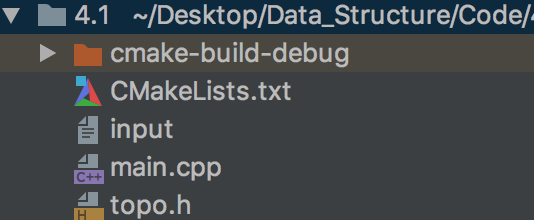
\includegraphics[width=0.8\textwidth]{41project.png}
\end{figure}

\newpage

2.依次点击菜单"Run"->build,再点击"Run",运行程序。

\begin{figure}[h]
    \centering
    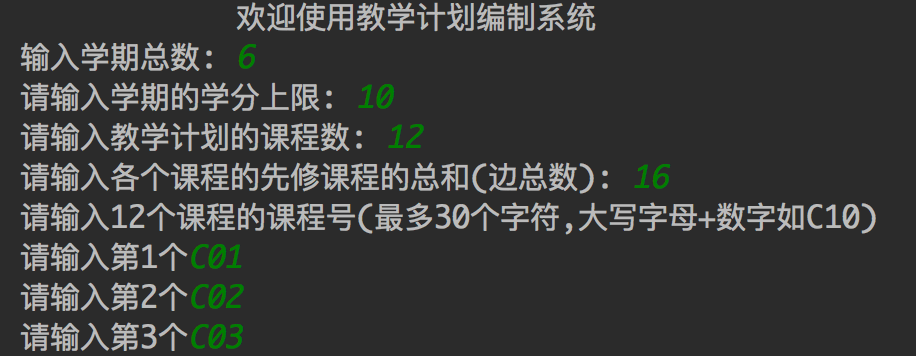
\includegraphics[width=0.8\textwidth]{interface41.png}
\end{figure}



3.输入用户自定义的信息后输出结果。

\section{测试结果}

在输入测试数据后,生成以下文件内容。

\begin{figure}[h]
    \centering
    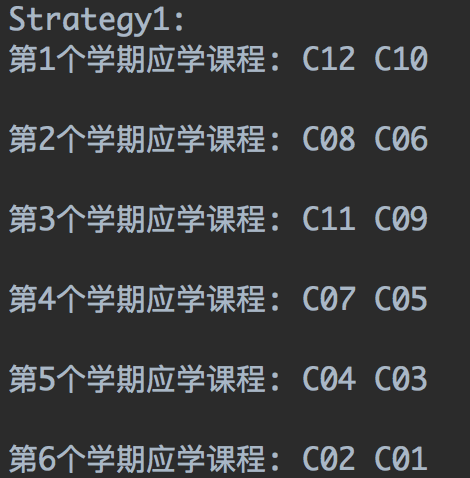
\includegraphics[width=0.4\textwidth]{result41.png}
\end{figure}

	根据以上测试结果数据分析,可以得出模拟数据与理论时间复杂度相符。

\section{附录}

源程序文件名清单

main.cpp               \qquad \quad  //主函数

topo.h            \qquad \qquad //排序函数单元模块



\end{document}




